% DUET -- Implementation (DAC 2027 draft, 2026-11-07)
% Code: nvmevirt/ (snapshots of ~/nvmevirt_<policy>, README.md), shared glue dm_ftl.c, FTLs under dm/ftl_*.c.
% Shared changes vs upstream: host-read priority with program/erase suspend (ssd.c), credit-paced background NAND ops and
% staged-write buffer accounting (dm_ftl.c), admin Identify PRP fix (admin.c), OP 7% geometry (ssd_config.h).
% Each FTL was first written in the trace-driven simulator (ftlsim) and ported, bit-identical on the validation traces.
% ftl_proposed.c = 1559 lines. Baseline params: tools/apps/common.sh (*_vb aliases).

% Fig. 5 and 6 (eval read / write) are defined here so that they float to the top of page 5.
\begin{figure*}[t]
  \centering
  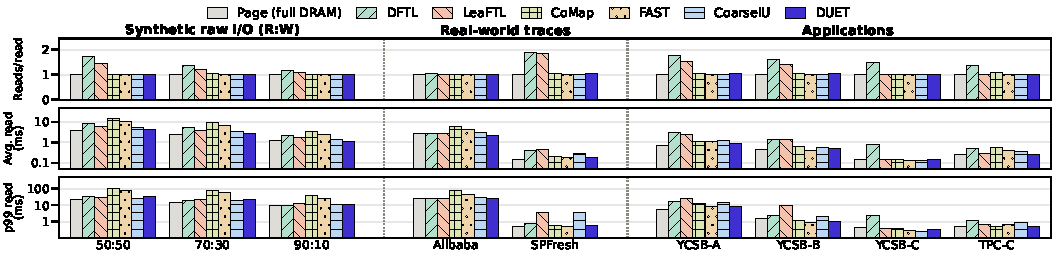
\includegraphics[width=\textwidth]{figs/fig_eval_read.pdf}
  \vspace{-6mm}
  \caption{Read path. From top, flash reads per host read (data plus mapping reads), and average and p99 read latency.}
  \label{fig:eval-read}
  \vspace{-2.5mm}
\end{figure*}

\begin{figure*}[t]
  \centering
  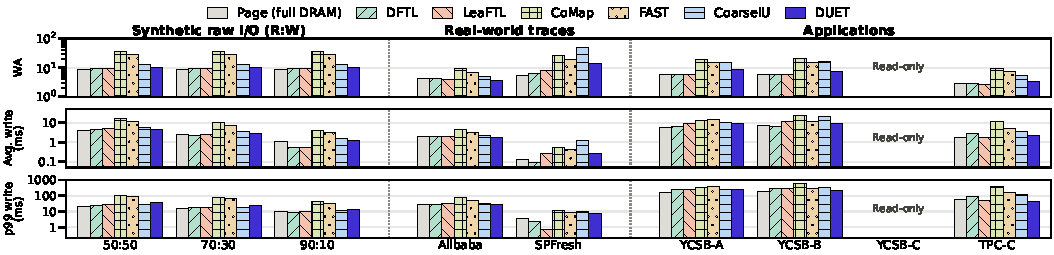
\includegraphics[width=\textwidth]{figs/fig_eval_write.pdf}
  \vspace{-6mm}
  \caption{Write path. From top, device write amplification, and average and p99 write latency. YCSB-C is read-only.}
  \label{fig:eval-write}
  \vspace{-2.5mm}
\end{figure*}

\section{Implementation}
\label{sec:impl}

We implement DUET and six other FTLs in NVMeVirt~\cite{nvmevirt}, a kernel-level
NVMe SSD emulator that models the latency of every NAND read, program, and erase
over its channels and dies. We add a common FTL interface to NVMeVirt. Each FTL
implements the host read, write, and flush handlers and its own GC, and it issues
every data and mapping access as a flash operation. Mapping reads and programs
therefore take NAND time like data accesses and are counted in WA. All FTLs share
the same NAND model, write buffer, and host interface and differ only in the FTL.
Based on the NVMeVirt code, we also let host reads suspend programs and erases and
pace background NAND operations to mimic real SSDs. These changes apply equally to
all FTLs. DUET takes about 1,600 lines of C.
